\section{An answer for Question \ref{q:why}: The cause of measurement clusterization}\label{section:why}
\begin{figure}[H]
    \centering
    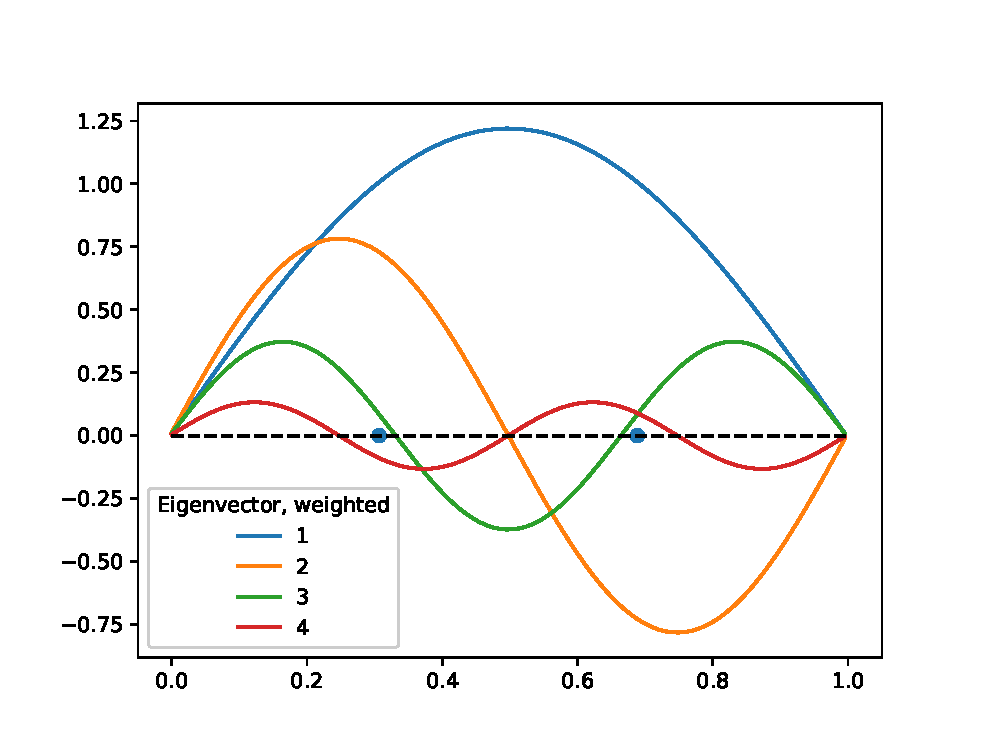
\includegraphics[height=0.5\textwidth]{eigenvectors.eps}
    \caption{D-optimal measurement locations ($m=5$ measurements) and
      weighted eigenvectors for inversion of the initial condition of
      the 1D heat equation (see supplementary material for
      details). Measurement locations and weighted eigenvectors are
      plotted over the computational domain $\Omega = [0, 1]$
      (x-axis).  Measurement clusterization occurs approxmately at
      $0.31$ and $0.69$. These two locations are a compromise between
      zerosz of the irrelevant eigenvectors (third and up) and staying
      far from a zero of the first and second eigenvectors.}
  \label{fig:why}
\end{figure}


According to Theorem \ref{thm:char}, D-optimal designs aim to measure
a small subset of eigenvectors; namely, eigenvectors $1$ through
$k$. In our model, not measuring eigenvectors $k+1$ and above is
readily achieved, as the proof of Theorem \ref{thm:char} demonstrates.
Taking this understanding to spatial problems, we expect a D-optimal
design to prefer measurement locations where eigenvectors $k+1$ and
above are (close to) zero: either because their eigenvalue in the
spectrum of the prior is small, or because the value of the
eigenvector itself is (close to) zero. Figure \ref{fig:why}
demonstrates this preference for the 1D heat equation with homogeneous
Dirichlet boundary conditions (details in the supplementary
material). We plot four eigenvectors, scaled according to their prior
standard deviations. We ignore eigenvectors above the fourth, due to
their small prior eigenvalues. We can observe that measurements are
clustered close to zeros of the third and fourth eigenvectors. The
reason for this measurement clusterization is that there are only two
locations where the third and fourth eigenvectors are close to zero,
and the first and second eigenvectors are considerably larger than
zero. When we fit four measurements into these measurement locations,
we find that measurements cluster, in accordance with the pigeonhole
principle.


%% \textbf{Question \ref{q:why}}:
